%%%%%%%%%%%%%%%%%%%%%%%%%%%%%%%%%%%%%
% IEEES 2020 conference FORMAT checklist:
% - to check!
% FORMAT: 
%            - roman numbers for sections, how do I change it?
%            - fix references parenthesis style (see notes in reference section)
%
%
%
% CHECKLIST/TODO:
% - real case graphs data/spikes
% - heating strategy and setpoint (add power to the graph)
%
%%%%%%%%%%%%%%%%%%%%%%%%%%%%%%%%%%%%%%



%Fonts are typically available only in certain sizes/increments. As an example, the basic article document class loads only the following sizes (from size10.clo):

 %   \tiny @ 5pt;
 %   \scriptsize @ 7pt;
 %   \footnotesize @ 8pt;
 %   \small @ 9pt;
 %   \normalsize @ 10pt;
 %  \large @ 12pt;
 %   \Large @ 14.4pt;
 %   \LARGE @ 17.28pt;
 %   \huge @ 20.74pt; and
 %   \Huge @ 24.88pt


%%%%%%%%%%%%%%%%%%%%%%%%%%%%%%%%%%%%%%%%%%

\documentclass[10pt]{extarticle} %extendend font dimensions
\usepackage[margin=2cm,top=1cm,bottom=2cm]{geometry}
%\usepackage{helvet}
%\renewcommand{\familydefault}{\sfdefault}

%\usepackage[pass,showframe]{geometry}
\usepackage{amsmath}
\usepackage[english]{babel}
% author year bibliography  
\usepackage{natbib}

% Use of [T1]{fontenc}
% If you don't use \usepackage[T1]{fontenc}:
% - Words containing accented characters cannot be automatically hyphenated,
% - You cannot properly copy-and-paste such words from the output (DVI/PS/PDF),
% - Characters like the pipe sign, less than and greater sign give unexpected results.
\usepackage[T1]{fontenc}

\usepackage{newtxtext,newtxmath}

%%%%%%%%%% image packages:

\usepackage{graphicx}

\usepackage[export]{adjustbox}

\usepackage{subcaption}


%%%%%%%%%%%%%%%%%%%%%%%%%%

\renewcommand{\sfdefault}{phv} %makes arial the default font for sff

\newcommand{\bigsize}{\fontsize{12pt}{16pt}\selectfont} %12pt dim/ 16pt spacing

\newcommand{\subsecsize}{\fontsize{10pt}{10pt}\selectfont} %14pt dim 

\newcommand{\namesize}{\fontsize{10pt}{10pt}\selectfont} %13pt dim 

\usepackage[sf,pagestyles]{titlesec} % make section headings \sffamily

% headings formats:

\titleformat{\section}[block]
            {\sffamily\normalsize\bfseries}
            {\thesection.}{6pt}{\filright}
            
\titleformat{\subsection}[block]
            {\sffamily\subsecsize\bfseries}
            {\thesubsection.}{6pt}{\filright}

\titleformat{\subsubsection}[block]
            {\sffamily\subsubsecsize\bfseries}
            {\thesubsubsection.}{6pt}{\filright}

%% https://tex.stackexchange.com/questions/326331/titleformat-problem


%title format:-----------------------
\usepackage{titling} % make titling elements \sffamily
\pretitle{\begin{center}\sffamily\bigsize\textbf}
\preauthor{\begin{center}
            \small\sffamily\ \lineskip 0.5em%
            \begin{tabular}[t]{c}}
%------------------------------------

% abstract format:-------------------
\usepackage{abstract}
% make abstract title \sffamily

\renewcommand\abstractnamefont{\sffamily\normalsize\bfseries}
\renewcommand{\abstracttextfont}{\sffamily\normalsize}
\renewcommand{\absnamepos}{raggedleft}
\setlength{\absleftindent}{0cm}
\setlength{\absrightindent}{0cm}

% ------------------------------------

%\bibliographystyle{vancouver}
\bibliographystyle{plainnat}

\title{The dead state of buildings}
\author{Valentina Bonetti\\ University of Strathclyde, Department of Mechanical and Aerospace Engineering, 75 Montrose St, Glasgow, G1 1XJ,  UK\\ \\ E-mail: valentina.bonetti@strath.ac.uk}

\date{}

% NOTES ABOUT ARTICLE CONTENT:

% - REFER	 to SalaLizarraga2020 chapter of book for summary of meaning and ref environment requirement (part of the problem or background)

% keep reading WEPFER GAGGIOLI 1979-80 "Reference datums for available energy"


\begin{document}
\renewcommand{\abstractname}{Abstract:}



\begin{figure}[!h]
\centering
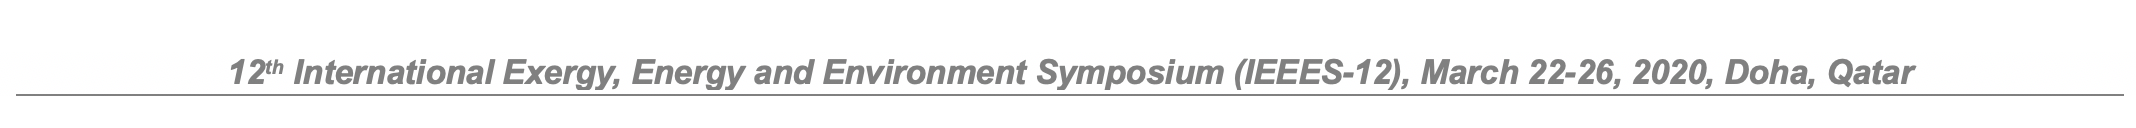
\includegraphics[width=6.8in, center]{images/articleHeading1.png}
\end{figure}

%\maketitle
\let\newpage\relax
\vspace*{-2cm}
\maketitle
\vspace*{-1cm}


\begin{abstract}

\noindent Exergy is typically defined as the maximum work that can be extracted from a system when reaching equilibrium with its ``reference environment'' - a large region unaffected by the interactions - and derives from Gibbs' original concept of ``available energy of a body and medium''. The reference environment definition  plays a key role in exergy analysis but is still controversial, especially in the case of buildings; the most popular choice is the local outdoor air, because readily available and largely unaffected by the presence of the building, but its fluctuating conditions pose various challenges. The controversy around the reference environment arguably remains one of the main blockers in the practical application of building exergy methods.
However, going back to the origins, Gibbs defined available energy not only for a ``body and medium'', but also for the case of a ``body alone'', a system formed by subsystems in non-equilibrium conditions. Later, exergy too was defined for this second case, as the subsystem contribution to the body available energy. In the case of the ``body alone'', the reference is the ``dead state'' (the thermostatic condition of the body), in place of the reference environment. 
The main idea of this article is that building exergy analysis can be based not only, as currently, on the exergy definion originated by Gibbs' case of the ``body and medium'', but alternatively on the exergy definition originated by the case of the  ``body alone'', for which a large environment is not needed.  The outdoor reference environment can thus be substituted by an indoor ``dead state''. 
The study discusses possible system boundaries and ways of defining the building dead state based on indoor conditions, and the potential impact on building exergy analysis. The dynamic exergy modelling of a few cases is presented to visualise the numerical implications.

\end{abstract}

\noindent {\sffamily\normalsize\bfseries Keywords:}
{\sffamily\normalsize Exergy, reference environment, dynamic analysis.}


\section{Introduction} 

\sffamily\normalsize

% SUGGESTIONS:
%Help the reader understand why your research is important and what it is contributing to the field:
%Start by giving the reader a brief overview of the current state of research in your subject area.
%Progress to more detailed information on the specific topic of your research.
%End with a description of the exact question or hypothesis that your paper will address.
%Also state your motivation for doing your research and what it will contribute to the field.

%The problem
Building exergy analysis is an interesting concept, but it is hardly applied or even known in practice. The controversy on the reference state definition, the complexity of the analysis and the lack of convincing practical benefits are possibly the biggest obstacles to its utilisation. In the author's opinion, the main problem is the adoption of the varying outdoor ambient conditions as the reference state. First of all, outdoor fluctuations, combined with the inertia of the building envelope, make the outdoor environment not as directly available as claimed; secondly, the meaning of ``warm" and ``cool" exergies based on the variable outdoor temperature can be misleading, especially because they are often treated as if they were always usable for heating and cooling respectively. For instance in \cite{Choi2020} (left colum of page 11), energy stored at 25$^\circ C$ is proposed as cool exergy useful for indoor cooling when the outdoor temperature is 30$^\circ C$, and energy stored at 15$^\circ C$ degrees is considered as warm exergy that could be used for indoor heating when the outdoor temperature is 10$^\circ C$, in a case where the indoor temperature is 20$^\circ C$; this is misleading because just defining something ``warm" or ``cool" because it is less cold or less hot than the outdoor conditions does not necessarily make it useful for heating or cooling (at most for some limited fresh air pretreatment). As already observed in \cite{Bonetti2016} and \cite{Bonetti2017a}, where the benefits of having an exergy reference based on indoor conditions are discussed, defining warm and cool exergies on the base of outdoor variable conditions is not compatible with the common meaning of ``warm" and ``cold" and cannot be directly translated into heating or cooling fluxes.
%%%%%%%%%%%%%%%%%%%%%%%%%%%%%%%%%%%%%%%%%%%%%%%%%%%
%%%% CHECK and write down exact temperatures and write source to the Choi2020 graph
%%%%%%%%%%%%%%%%%%%%%%%%%%%%%%%%%%%%%%%%%%%%%%%%%%%
% complete problem section

%%%%%%%%%%%%%%%%%%%%%%%%%%%
%
%
%


% The idea
One alternative to variable outdoor air conditions is the use of indoor conditions. In the past, indoor air has been considered as a reference state for building exergy analysis, and the main argument against its use has been the fact that indoor air is not a large environment, as required by the definition of exergy \citep{Schmidt2011}. But where did this requirement come from? Answering this question requires going back to the origins.

% Gibbs
\cite{Gibbs1873} was the first to incorporate the first and second law of thermodynamics in one equation \citep{Klein1990}, in his paper "Graphical Methods in the Thermodyna\-mics of Fluids".  The combination of the first and second law led Gibbs to introduce the concept of ``available energy"; he distinguished two cases: a "body alone", in internal non-equilibrium conditions, and a "body and medium", in non-equilibrium conditions with each other. 

In the case of the ``body alone", the available energy of the body is the greatest amount of mechanical work that ideally can be obtained by taking the body, without any net contributions of energy from external objects, from the initial non-equilibrium condition to its point of stable or neutral equilibrium (on its ``surface of dissipated energy") that has the same entropy and volume of the initial state. The internal non-equilibrium state of the body can assume various forms, like a difference in the pressure of some of its part, or a gradient in temperature, or even different chemical compositions. It is important to observe that the term ``body" refers not necessarily to a single entity but to a system that is potentially including several subsystems and processes \citep{Gaggioli2012}.
 
In the case of the ``body and medium", the medium is supposed to be at uniform pressure and temperature and it is defined as ``reference environment": a large subsystem that is not affected by the interactions with the other components of the overall system, and is represented by a plane in Gibbs' energy-entropy-volume space. The available energy in this case is the distance (on the energy axis) from the point corresponding to the initial conditions of the body to the point with the same entropy and volume on the reference plane. Even if the body is in internal equilibrium, the combination between body and medium can still have available energy, unless they are in the same conditions. 


%Present some of fundamental Gaggioli equations for exergy.
The vast majority of exergy analysis is based on the second case, the  ``body and medium", and relies on the definition of a reference environment (the medium). However, \cite{Gaggioli2012} examined in depth the meaning of ``dead state" and highlighted that exergy can be based on Gibbs' ``available energy of a body" (the first case mentioned above), which does not require a reference environment. The exergy of each subsystem of an overall system (in which no large one is required) was defined by \cite{Gaggioli1998} as the subsystem contribution to the available energy of the overall system, with the reference being the overall system ``dead state" - its thermostatic conditions, where all the sub-parts are in equilibrium, subject to the given constraints. Such subsystem exergy is additive, and exergy balances can be used to perform exergy analysis. According to \cite{Gaggioli2012}, If subsystems are free to exchange entropy $S$ and volume $V$, the exergy content $Ex_i$ of each subsystem $i$ is $Ex_i = E + p_f - T_fS$, where the subscript $f$ indicates the dead state.

The main idea of this study is that building exergy analysis can be based on Gibbs' case of the ``body alone" and does not require a large environment, but can rather use, as the reference state, a definition of dead state related to indoor comfort. In order to make the ``body alone" relevant to building design, its boundaries include the indoor air and all the inner parts of the envelope that have a direct impact on indoor conditions (in practice, the depth of thermal mass that effectively contributes to the envelope interior storage). The dead state here proposed as a reference is a fixed ``target comfort" state, in order to avoid all the problems linked to reference fluctuation described by \cite{Pons2009}. This choice would make the definition of ``warm" and ``cool" exergies more straightforward to understand and relevant to heating and cooling strategies. The article discusses how different the proposed model is from Gibbs' case of the ``body alone", how distant the actual dead state of such system could be from a fixed comfort target, and what impact the discrepancies could have on exergy design and control strategies based on this reference.

\section{The dead state of a ``box" building} \label{subsec:simple}


%Discuss an insulated cave with no air exchanges and negligible internal gains. Simulate it on the side and present image.


 
\begin{figure}[h]
 
\begin{subfigure}{0.35\textwidth}
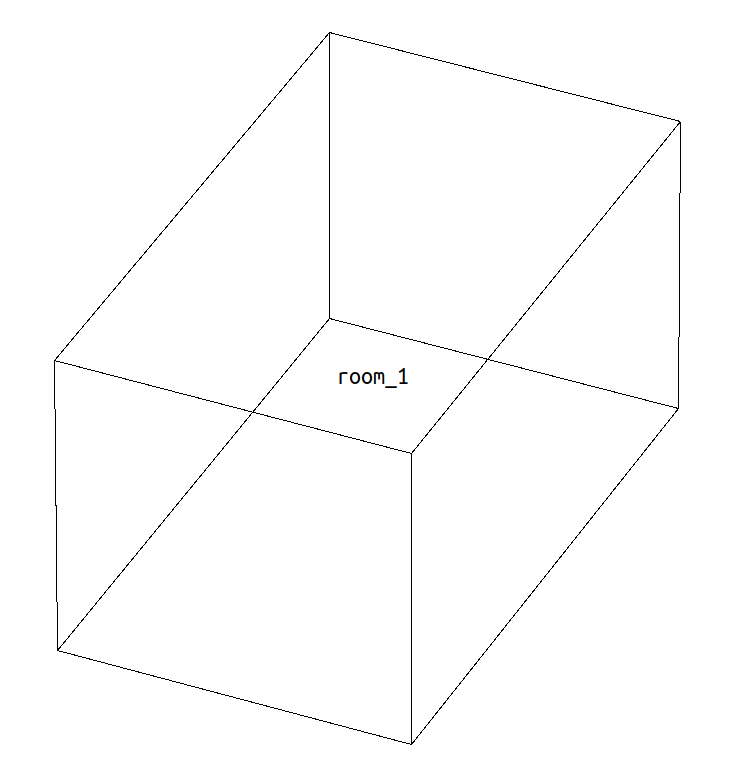
\includegraphics[width=0.95\linewidth, height=6cm]{images/Dead02_boxModel.png} 
\caption{ESP-r box model.}
\label{fig:esprmodel}
\end{subfigure}
\begin{subfigure}{0.65\textwidth}
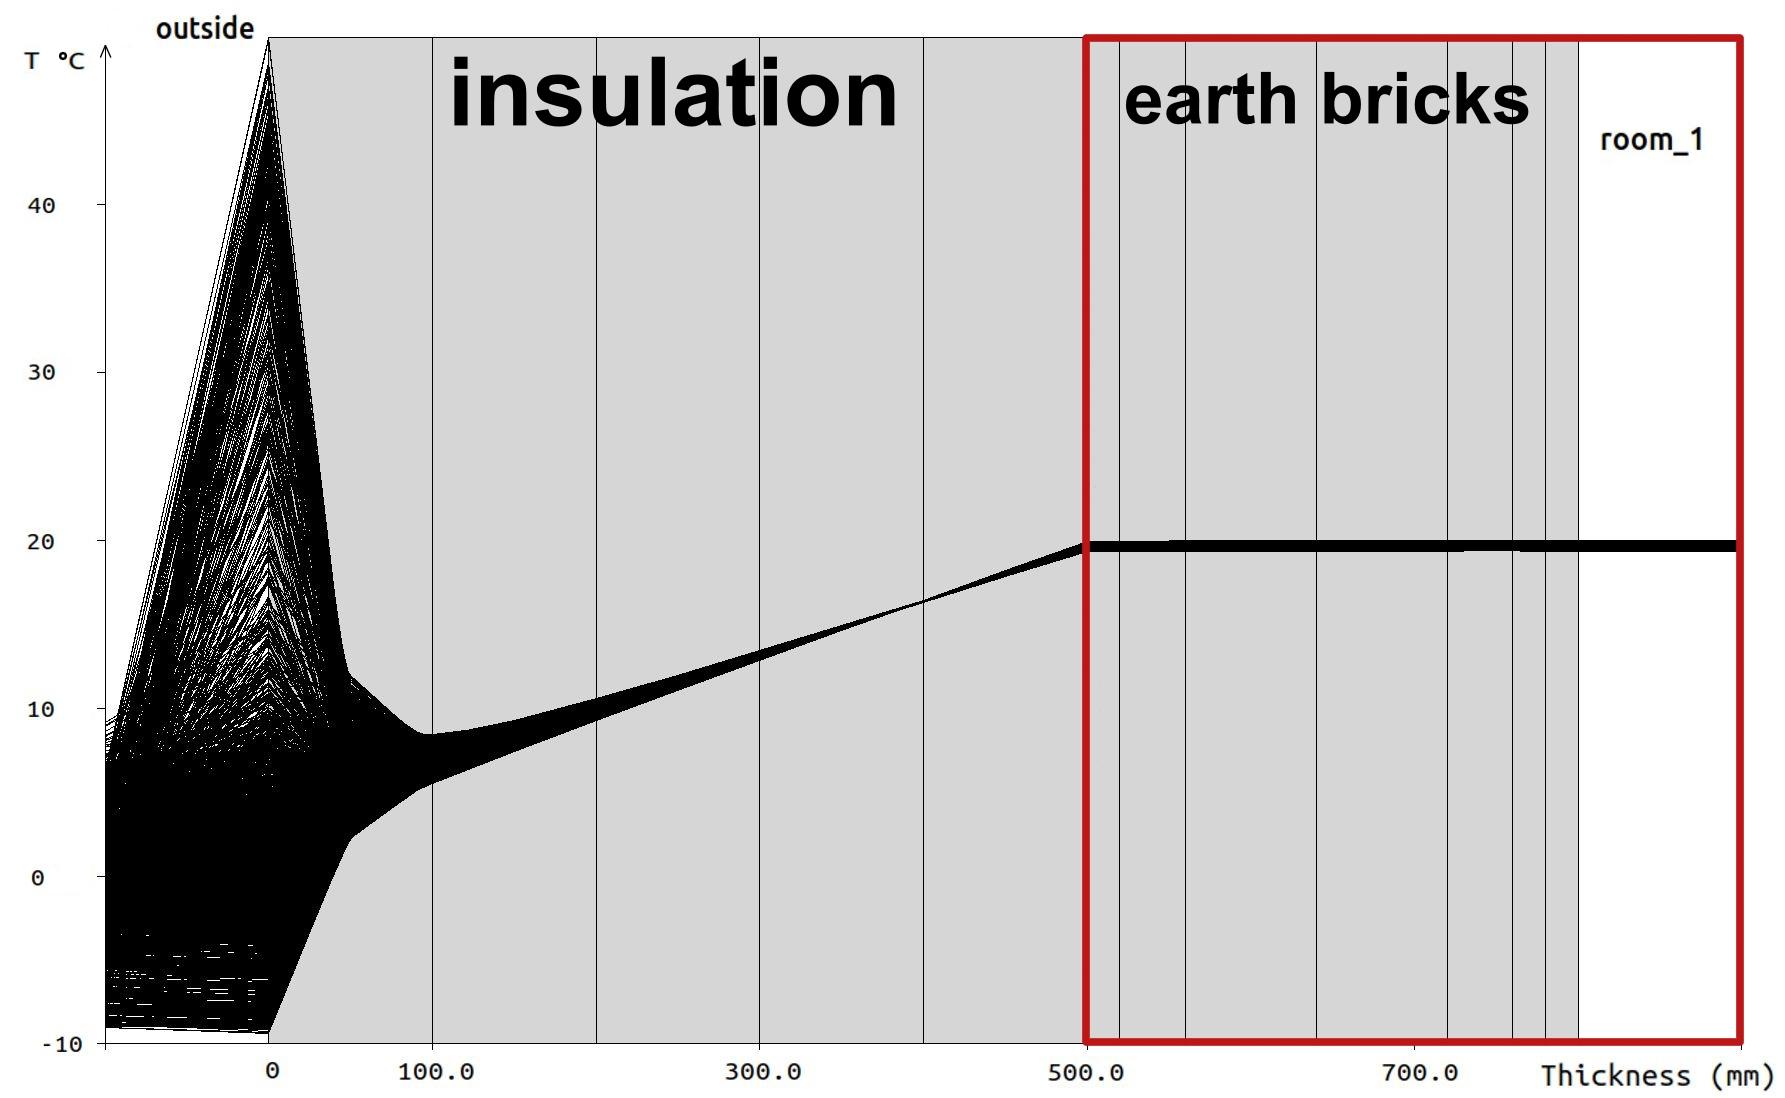
\includegraphics[width=0.95\linewidth, height=6cm]{images/01Feb_28Feb_Wall1_dead02_krita.jpg}
\caption{Cumulative values of intra-construction temperatures in a wall of the box model.}
\label{fig:constructionelements}
\end{subfigure}
 
\caption{The first case study: a box model with 500 mm of high  insulation and 300 mm of earth on the internal layers.}
\label{fig:casestudy}
\end{figure}


\vfill \break




\section{Internal conditions of realistic cases} \label{subsec:moreComplex}

...although this system is not actually closed and isolated, especially in buildings with lower performances,  ... transmission losses are low for good envelopes and fresh air intakes are controlled or known, which makes them considerable as a subsystem added to indoor air.

Statement about the importance of internal loads, not only for summer but also on heating strategies. Define the "core" of the envelope (periodic penetration depth) and specify that it is a first attempt definition.
Calculate instantaneous dead state and compare with target dead state: $T_{eq}={\sum_i m_i c_i T_i} / {\sum_i m_i c_i}$

%\begin{equation}
%T_{eq}={\sum_i m_i c_i T_i} / {\sum_i m_i c_i}
%\end{equation}


\begin{figure}[h]
 
\begin{subfigure}{0.5\textwidth}
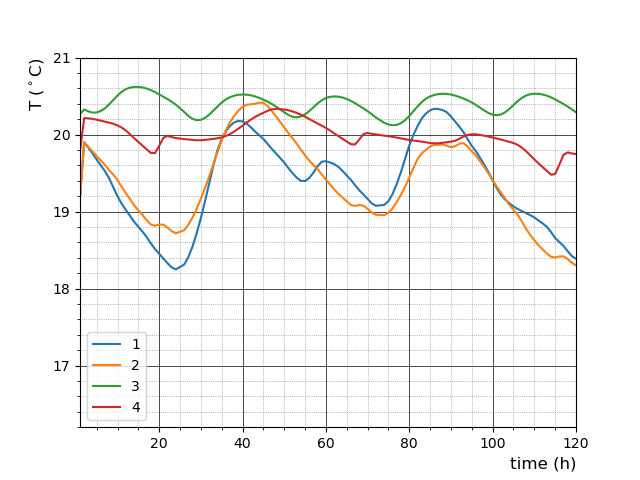
\includegraphics[width=0.99\linewidth, height=7cm]{images/1.png} 
\caption{Radiant wall heating}
\label{fig:esprmodel}
\end{subfigure}
\begin{subfigure}{0.5\textwidth}
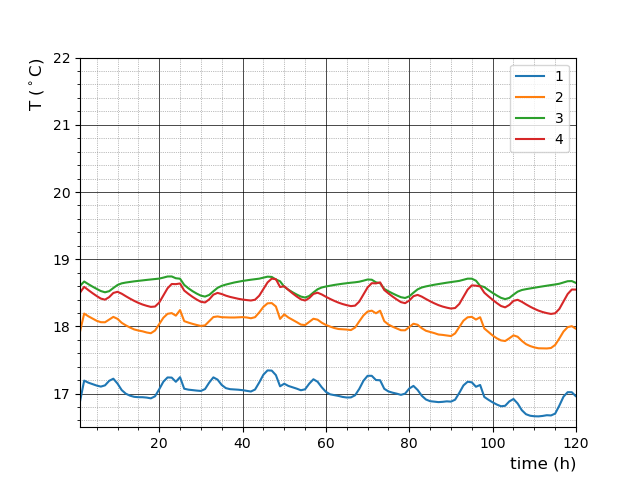
\includegraphics[width=0.99\linewidth, height=7cm]{images/2.png}
\caption{Basic ideal heating (air node heat injection)}
\label{fig:constructionelements}
\end{subfigure}
 
\caption{The thermostatic temperature of four different thermal zones of a realistic flat (5-day period in February, UK climate).}
\label{fig:casestudy}
\end{figure}

\section{Thermal exergy sensitivity}

Formula of sensitivity and explain the graph:

\begin{equation}
\sigma =  {Ex(T0+\Delta T0)-Ex(T0) \over Ex(T0)} = { { Q \left( 1-{T0+ \Delta T0 \over T} \right) } - { Q \left( 1-{T0 \over T} \right) } \over { Q \left( 1-{T0 \over T} \right) } } = { \Delta T0 \over T0 - T }
\end{equation}

\begin{figure}[h]
 
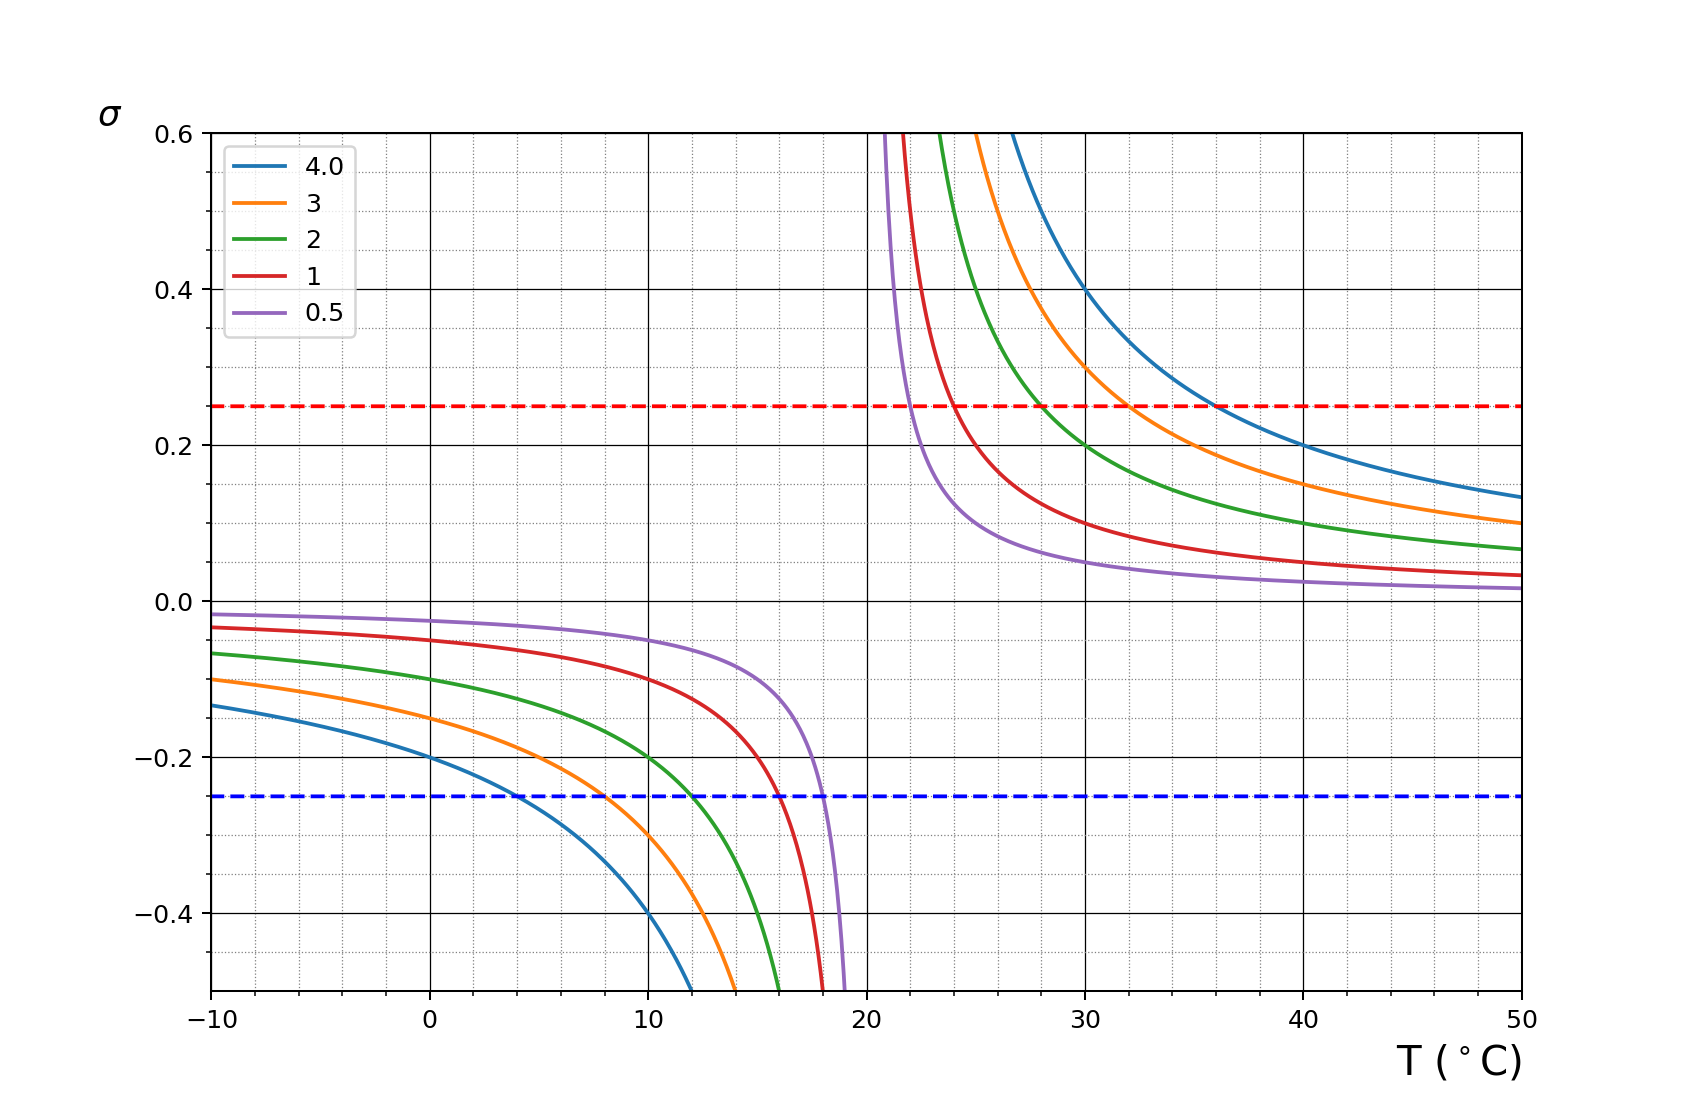
\includegraphics[height=8.5cm, center]{images/sensitivity.png} 

\caption{The first case study: a box model with 500 mm of exterior  insulation and 300 mm of earth on the internal layers.}
\label{fig:casestudy}
\end{figure}

\vskip3cm

\section{Dead state and design goals}

%state why you want the reference state to be fixed (cite Pons 2019)
\cite{Pons2019} 

In most cases the core of the building envelope is far from an isolated system, but the indoor environment has a comfort target nevertheless. When the HVAC system is switched off, we expect the indoor conditions to remain comfortable for as long as possible, and as soon as they fall out of an acceptable range the heating or cooling system intervenes again to bring temperature and sometimes also relative humidity back to the required values. In other words, it is like if the composition of the overall system changed dynamically to include subsystems capable of re-establishing the desired dead state. Sometimes the external environment has the exergy that the building needs to maintain its conditions, for instance cooler air could be let in to readdress internal gains, or solar radiation could enter from fenestration to compensate transmission losses. When the balance cannot be maintained by passive design strategies, an exergy input from renewable or non-renewable sources is required. In any case, the final destination is an indoor environment very close to, or going towards, comfort conditions, with a multitude of exergy fluxes and storages being orchestrated to balance each other with the goal of a comfortable dead state.

The core of the building, including the internal part of the envelope and the indoor environment, might have both warm and cool exergy storages, which both contribute to the overall exergy, in this case also "available energy". A greater available energy is an expression of disequilibrium, and potentially of a greater effort needed to maintain comfort conditions. Zero available energy indicates that the system is in uniform comfort conditions, because all the exergy contributions are positive.





\section{Conclusions and future work}
Wall insulation is relatively easy - main challenges today are indoor comfort and thermal storage / decoupling energy demand and offer (just my opinion though, look for references). Indoor dead state shifts the focus on the indoor environment.

\section*{Acknowledgments}

The author thanks the Engineering and Physical Sciences Research Council U.K. (EPSRC, Grant No.1586601) and the Building Research Establishment (BRE) for the financial support.

{\small %font size 9
 \bibliography{ValeIEEES2020}
}
%% Max 10-15 refs
% NOTES FOR BIBLIOGRAPHY
% References“Arial, 10 points, bold”
% “Arial, 9 points, alphabetic order of names (first author), max 10-15 important references.”
% “If Mendeley is used, you can select Journal of Cleaner Production or similar referencing styles”

\vfill \break



\end{document}




% LaTeX references:

% Use of package [T1]{fontenc}: 
% https://tex.stackexchange.com/questions/664/why-should-i-use-usepackaget1fontenc

% https://tex.stackexchange.com/questions/25249/how-do-i-use-a-particular-font-for-a-small-section-of-text-in-my-document

% abstract package documentation:
% http://citeseerx.ist.psu.edu/viewdoc/download?doi=10.1.1.169.8953&rep=rep1&type=pdf

% title formats using titlesec:
% http://mirror.ox.ac.uk/sites/ctan.org/macros/latex/contrib/titlesec/titlesec.pdf
% https://tex.stackexchange.com/questions/326331/titleformat-problem

